\chapter{Rostliny, parametry a dělení skleníku na sekce}
Mluvíme-li o~malém pěstiteli, který pěstuje např. zeleninu pro svoji obživu, málokdy se stává, že by měl ve skleníku jen jeden typ rostlin (resp. monokulturu).
Ovšem vzhledem k~tomu, že každý typ rostliny má odlišné podmínky pro jejich pěstování, není možné bez speciálních úprav skleníku je libovolně kombinovat.
Díky PROTOPlantu je možno skleník rozdělit na zóny a pro každou nadefinovat vlastní parametry prostředí.
\newline

\noindent\B{Uvedu příklad:}

Mám velký skleník, ve kterém chci pěstovat papriky, rajčata, ale zároveň chci mít ve skleníku sekci, do které mohu přes léto zavěsit několik orchidejí.
Skleník tedy mohu rozdělit pomocí průchozí přepážky (závěsná fólie např. z~PVC) na dvě části, viz obrázek \ref{fig:separationA}.
V~PROTOPlantu poté pouze nastavím, které senzory se nacházejí v~které části.
Aktuátory pro okna od každé sekce připojím k~samostatným výstupům řídící jednotky (sekce A~k~výstupu č. 1, sekce B k~výstupu č. 2).
Díky tomu mohu parametry prostředí regulovat pro každou část samostatně.
Pro zavlažování poté stačí jedno čerpadlo a dva elektrické ventily, které budou regulovat průtok vody do jednotlivých částí.
\begin{figure}[htbp]
    \centering
    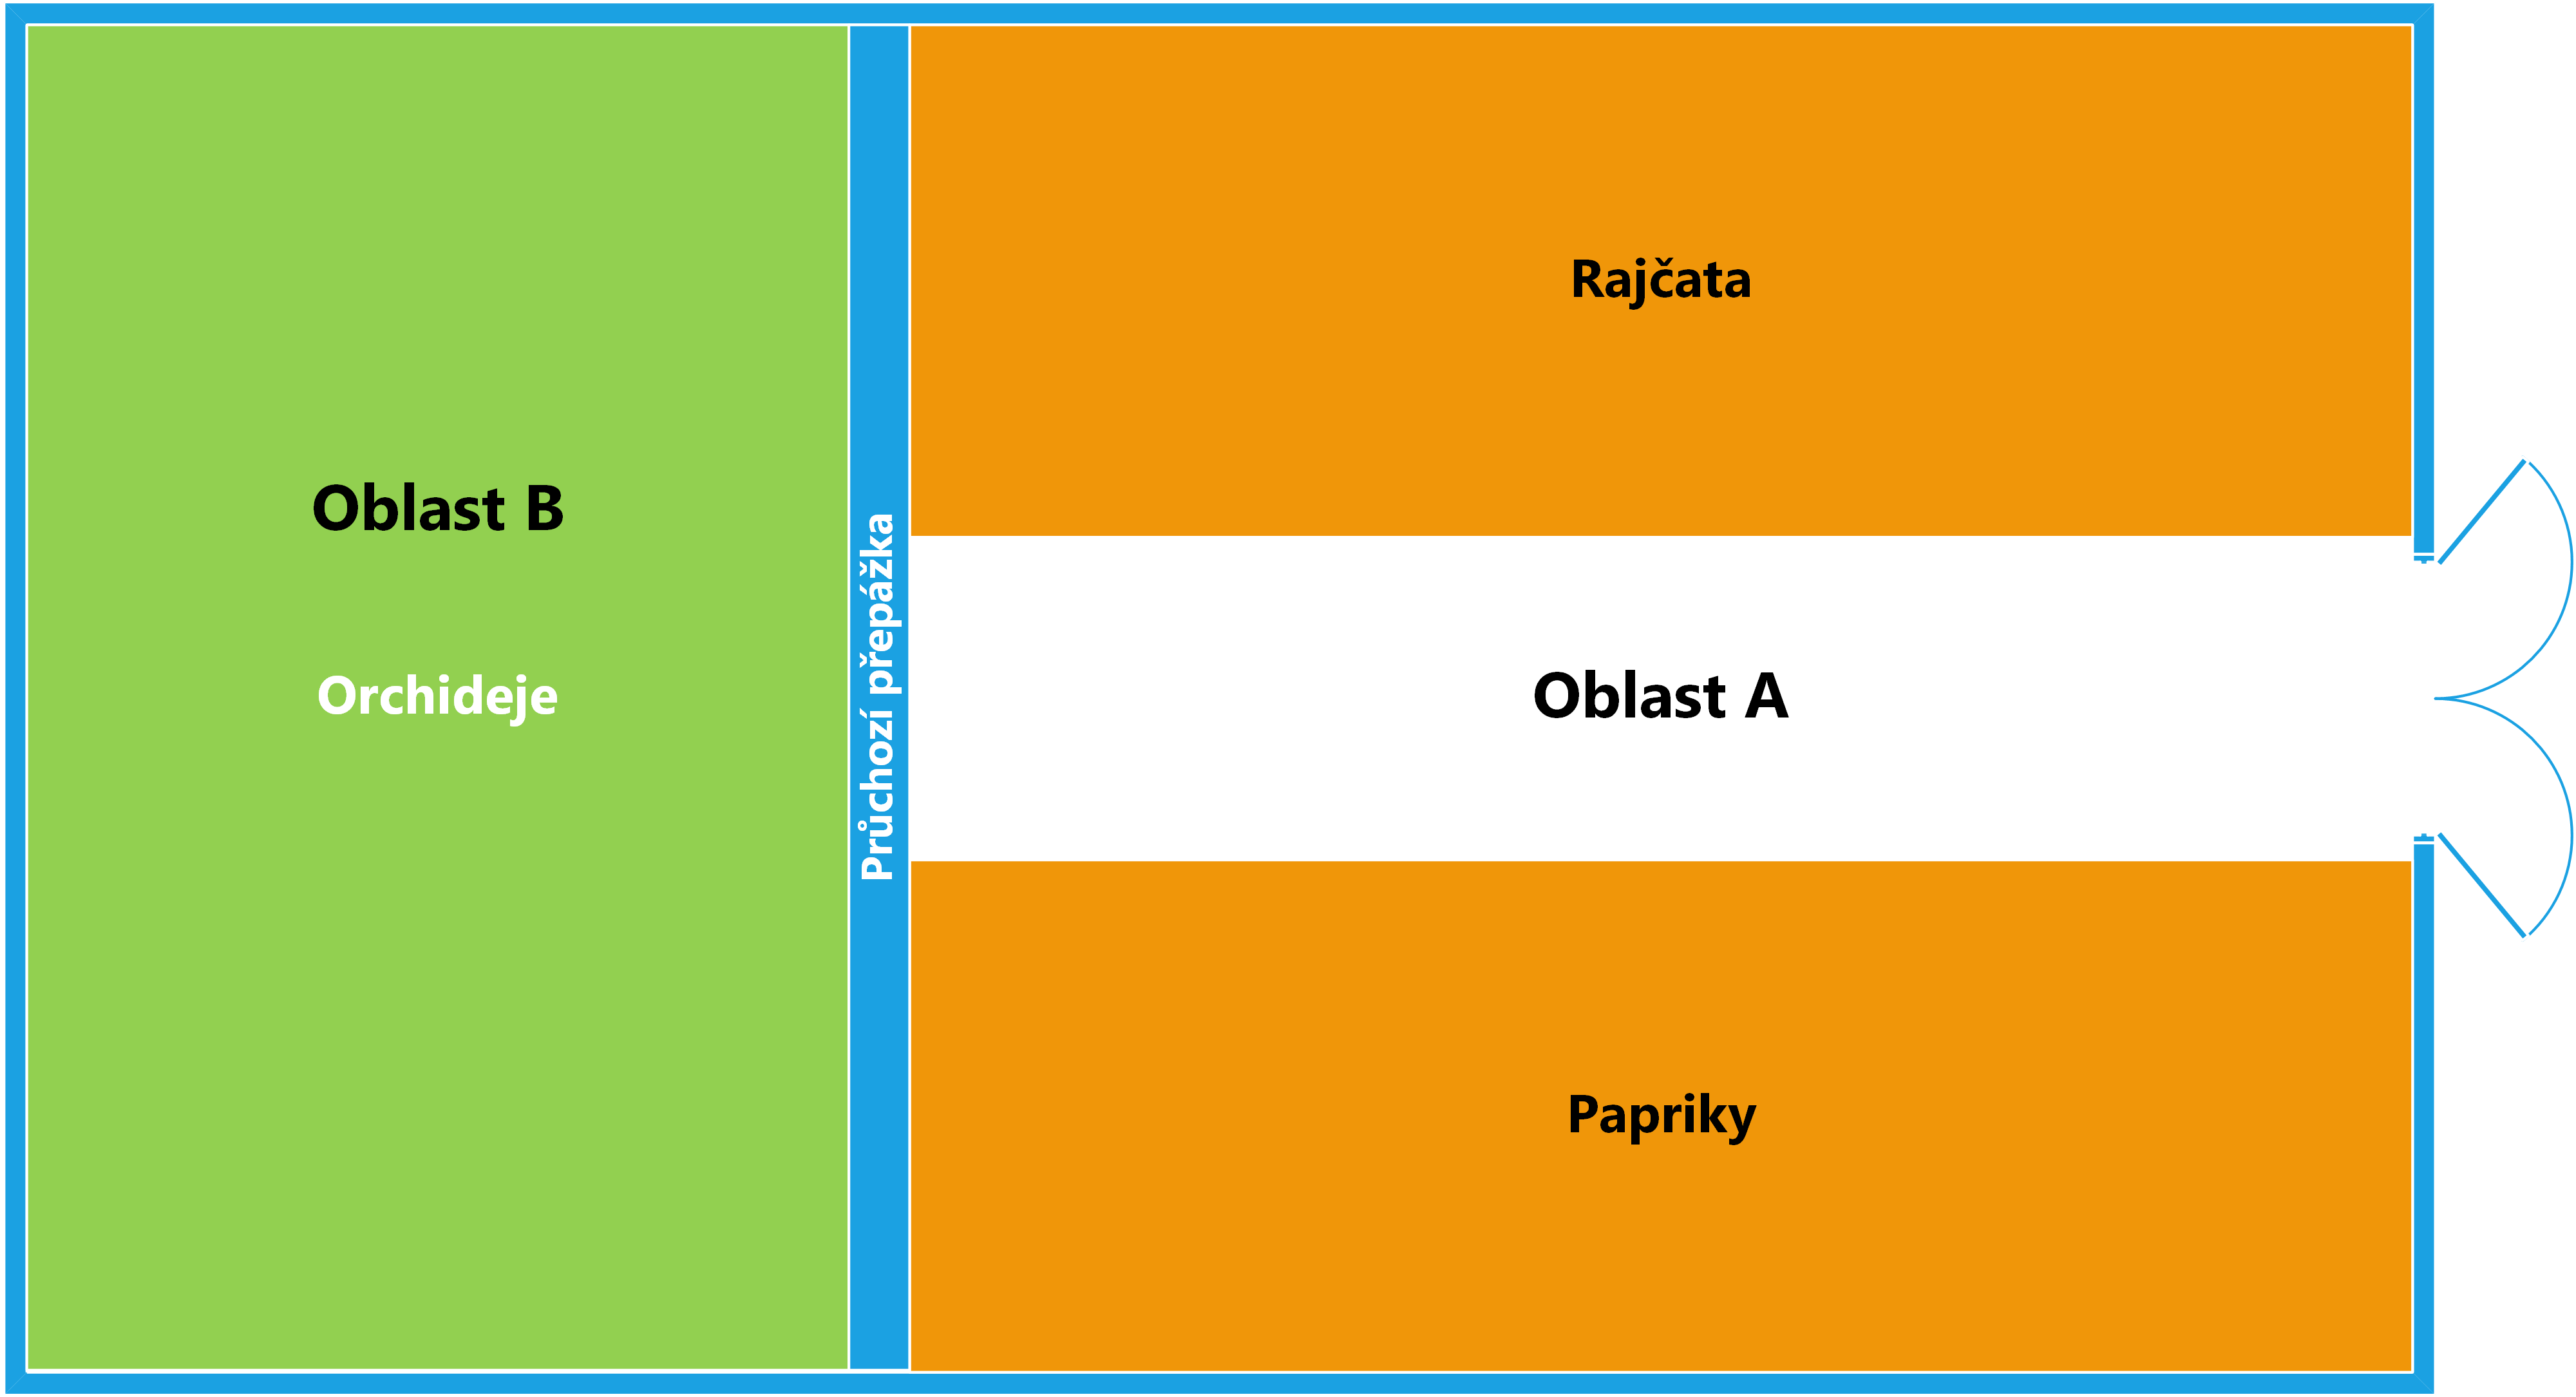
\includegraphics[width=0.85\textwidth]{img/Rozdeleni_Skleniku_A.png}
    \caption{Rozdělení skleníku na dvě oblasti.}
    \label{fig:separationA}
\end{figure}

Zároveň je takto možné testovat, jaké parametry jsou pro dané rostliny ideální a výsledky srovnat.
Pro tento účel mohu rozdělit skleník na poloviny se stejným typem rostlin a pro každou polovinu nastavit různé parametry.
Poté mohu velmi jednoduše sledovat výsledky.

\section{Přednastavení a režimy}
Do PROTOPlantu plánuji přidat několik přednastavených režimů pro parametry prostředí.
Uživatel tedy zasadí například rajčata a v~nastavení PROTOPlantu zvolí přednastavení „Rajčata“.
PROTOPlant automaticky změní hodnoty tak, aby podmínky vyhovovaly pěstování rajčat.
Pro zvolení nejlepších hodnot pro jednotlivá přednastavení plánuji navázat spolupráci s~odborníky.

\newpage